\begin{table}[h]
    \centering
    \begin{tabular}{cc}
      \begin{minipage}{0.45\textwidth}
        \centering
        \begin{tabular}{|l|c|}
          \hline
          \textbf{Zastávka} & \# \\ \hline
          Lesná, Haškova & 0 \\ \hline
          Brechtova & 1 \\ \hline
          Blažkova & 2 \\ \hline
          Arbesova & 3 \\ \hline
          Heleny Malířové & 4 \\ \hline
          Lesná, nádraží & 5 \\ \hline
          Štefánikova čtvrť & 6 \\ \hline
          Provozníkova & 7 \\ \hline
          Lesnická & 9 \\ \hline
          Zemědělská & 10 \\ \hline
          Černá Pole, Erbenova & 11 \\ \hline
        \end{tabular}
        \caption{Rozpis zastávok}
        \vspace*{\baselineskip}
        \begin{tabular}{|l|c|}
          \hline
          \textbf{Vstup} & \textbf{Hodnota} \\ \hline
          Kapacita vozidla & 80 \\ \hline
          Miest na sedenie & 30 \\ \hline
          Kompenzácia vozidla & 66,35 Kč \\ \hline
          Dĺžka trasy & 3,8 km \\ \hline
          Cena lístka & 25 Kč \\ \hline
        \end{tabular}
        \caption{Parametre vozidla a trasy}
      \end{minipage}
      \begin{minipage}{0.45\textwidth}
        \centering
        \begin{tabular}{|c|l|}
          \hline
          \textbf{h} & \textbf{Odchody} \\ \hline
          05 & 00, 10, 20, 30, 40, 50 \\ \hline
          06 & 00, 05, 10, 16, 21, 27, 32, 38, 43, 49, 54 \\ \hline
          07 & 00, 05, 10, 16, 21, 27, 32, 38, 43, 49, 54 \\ \hline
          08 & 00, 06, 12, 18, 24, 30, 36, 42, 48, 54 \\ \hline
          09 & 00, 08, 17, 25, 34, 42, 51 \\ \hline
          10 & 00, 07, 15, 22, 30, 37, 45, 52 \\ \hline
          11 & 00, 07, 15, 22, 30, 37, 45, 52 \\ \hline
          12 & 00, 08, 17, 25, 34, 42, 51 \\ \hline
          13 & 00, 10, 20, 30, 40, 50 \\ \hline
          14 & 00, 12, 24, 36, 48 \\ \hline
          15 & 00, 08, 17, 25, 34, 42, 51 \\ \hline
          16 & 00, 06, 12, 18, 24, 30, 36, 42, 48, 54 \\ \hline
          17 & 00, 05, 10, 15, 20, 25, 30, 35, 40, 45, 50, 55 \\ \hline
          18 & 00, 05, 10, 15, 20, 25, 30, 35, 40, 45, 50, 55 \\ \hline
          19 & 00, 06, 13, 20, 26, 33, 40, 46, 53 \\ \hline
          20 & 00, 08, 17, 25, 34, 42, 51 \\ \hline
          21 & 00, 12, 24, 36, 48 \\ \hline
          22 & 00, 20, 40 \\ \hline
        \end{tabular}
        \caption{Časový rozpis}
      \end{minipage}
    \end{tabular}
  \end{table}
  \begin{table}[h]
    \centering
    \begin{tabular}{|l|c|}
      \hline
      \textbf{Výstup} & \textbf{Hodnota} \\ \hline
      Počet príchodov cestujúcich & 11819 \\ \hline
      Počet prevezených cestujúcich & 11818 \\ \hline
      Počet neobslúžených cestujúcich & 1 (0,01\,\%) \\ \hline
      Celkový čas strávený čakaním & 46455 min \\ \hline
      Priemerný čas strávený čakaním & 4 min \\ \hline
      Celková kompenzácia & -29045 Kč \\ \hline
      Celkový zisk & 266405 Kč \\ \hline
      Priemerná spokojnosť cestujúcich & 97,14\,\% \\ \hline
      Celkový počet vozidiel & 144 \\ \hline
      Priemerná naplnenosť vozidiel & 20 (25,0\,\%) \\ \hline
    \end{tabular}
    \caption{Výstupy simulácie}
  \end{table}
  
  \begin{figure}[h]
    \centering
    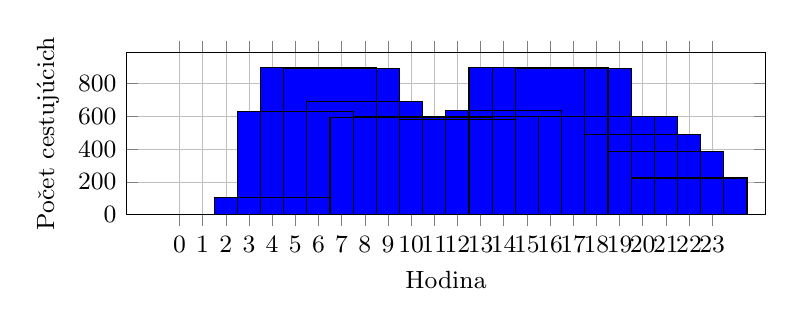
\begin{tikzpicture}
        \begin{axis}[
            width=0.8\textwidth,
            height=0.3\textwidth,
            xlabel={Hodina},
            ylabel={Počet cestujúcich},
            ymin=0,
            xtick={0,1,...,23},
            grid=both,
            major grid style={line width=.2pt,draw=gray!50},
            minor grid style={line width=.1pt,draw=gray!20},
            tick label style={font=\small},
            label style={font=\small},
            legend style={font=\small, at={(0.5,-0.2)}, anchor=north, legend columns=-1},
            ybar,
            bar width=5,
            ]
            \addplot[fill=blue] coordinates {
                (0, 0) (1, 0) (2, 0) (3, 0) (4, 106) (5, 630) (6, 901) (7, 891) 
                (8, 690) (9, 593) (10, 602) (11, 595) (12, 584) (13, 600) 
                (14, 636) (15, 898) (16, 898) (17, 893) (18, 601) (19, 599) 
                (20, 492) (21, 387) (22, 223) (23, 0)
            };
        \end{axis}
    \end{tikzpicture}
    \caption{Počet cestujúcich prichádzajúcich na zastávku za hodinu}
\end{figure}
\begin{figure}[h]
    \centering
    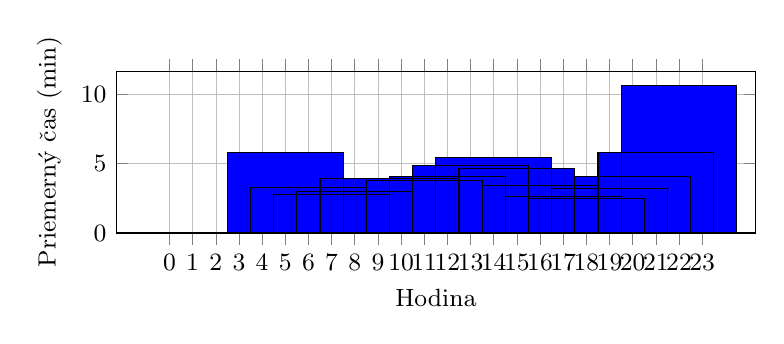
\begin{tikzpicture}
        \begin{axis}[
            width=0.8\textwidth,
            height=0.3\textwidth,
            xlabel={Hodina},
            ylabel={Priemerný čas (min)},
            ymin=0,
            xtick={0,1,...,23},
            grid=both,
            major grid style={line width=.2pt,draw=gray!50},
            minor grid style={line width=.1pt,draw=gray!20},
            tick label style={font=\small},
            label style={font=\small},
            legend style={font=\small, at={(0.5,-0.2)}, anchor=north, legend columns=-1},
            ybar,
            bar width=5,
            ]
            \addplot[fill=blue] coordinates {
                (0, 0) (1, 0) (2, 0) (3, 0) (4, 0) (5, 5.7936507936507935) (6, 3.2708102108768036) (7, 2.8002244668911334) 
                (8, 2.963768115942029) (9, 3.900505902192243) (10, 3.9385382059800667) (11, 3.7663865546218487) 
                (12, 4.087328767123288) (13, 4.888333333333334) (14, 5.411949685534591) (15, 4.6547884187082404) 
                (16, 3.4075723830734965) (17, 2.633818589025756) (18, 2.5058236272878536) (19, 3.2120200333889817) 
                (20, 4.09349593495935) (21, 5.767441860465116) (22, 10.596412556053812) (23, 0)
            };
        \end{axis}
    \end{tikzpicture}
    \caption{Priemerný čas strávený čakaním za hodinu}
\end{figure}
\begin{figure}[h]
    \centering
    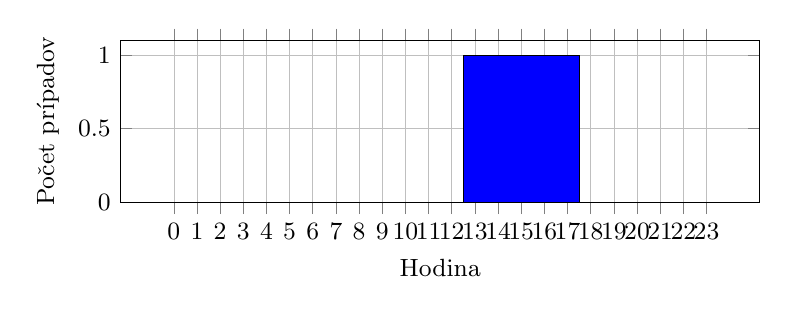
\begin{tikzpicture}
        \begin{axis}[
            width=0.8\textwidth,
            height=0.3\textwidth,
            xlabel={Hodina},
            ylabel={Počet prípadov},
            ymin=0,
            xtick={0,1,...,23},
            grid=both,
            major grid style={line width=.2pt,draw=gray!50},
            minor grid style={line width=.1pt,draw=gray!20},
            tick label style={font=\small},
            label style={font=\small},
            legend style={font=\small, at={(0.5,-0.2)}, anchor=north, legend columns=-1},
            ybar,
            bar width=5,
            ]
            \addplot[fill=blue] coordinates {
                (0, 0) (1, 0) (2, 0) (3, 0) (4, 0) (5, 0) (6, 0) (7, 0) 
                (8, 0) (9, 0) (10, 0) (11, 0) (12, 0) (13, 0) 
                (14, 0) (15, 1) (16, 0) (17, 0) (18, 0) (19, 0) 
                (20, 0) (21, 0) (22, 0) (23, 0)
            };
        \end{axis}
    \end{tikzpicture}
    \caption{Počet prípadov, kedy sa cestujúci nezmestili do vozidla za hodinu}
\end{figure}